\section{Neighborhood Analytics}
Neighborhood analytics aims to provide
summaries of each object over its vicinity. In contrast to aggregating the entire collection of data as a whole, neighborhood
analytic provides a personalized view for each object from its own perspective. Neighborhood
data analytics originates from the window function defined in SQL which is
illustrated in Figure~\ref{fig:window}.

\begin{figure}[h]
\centering
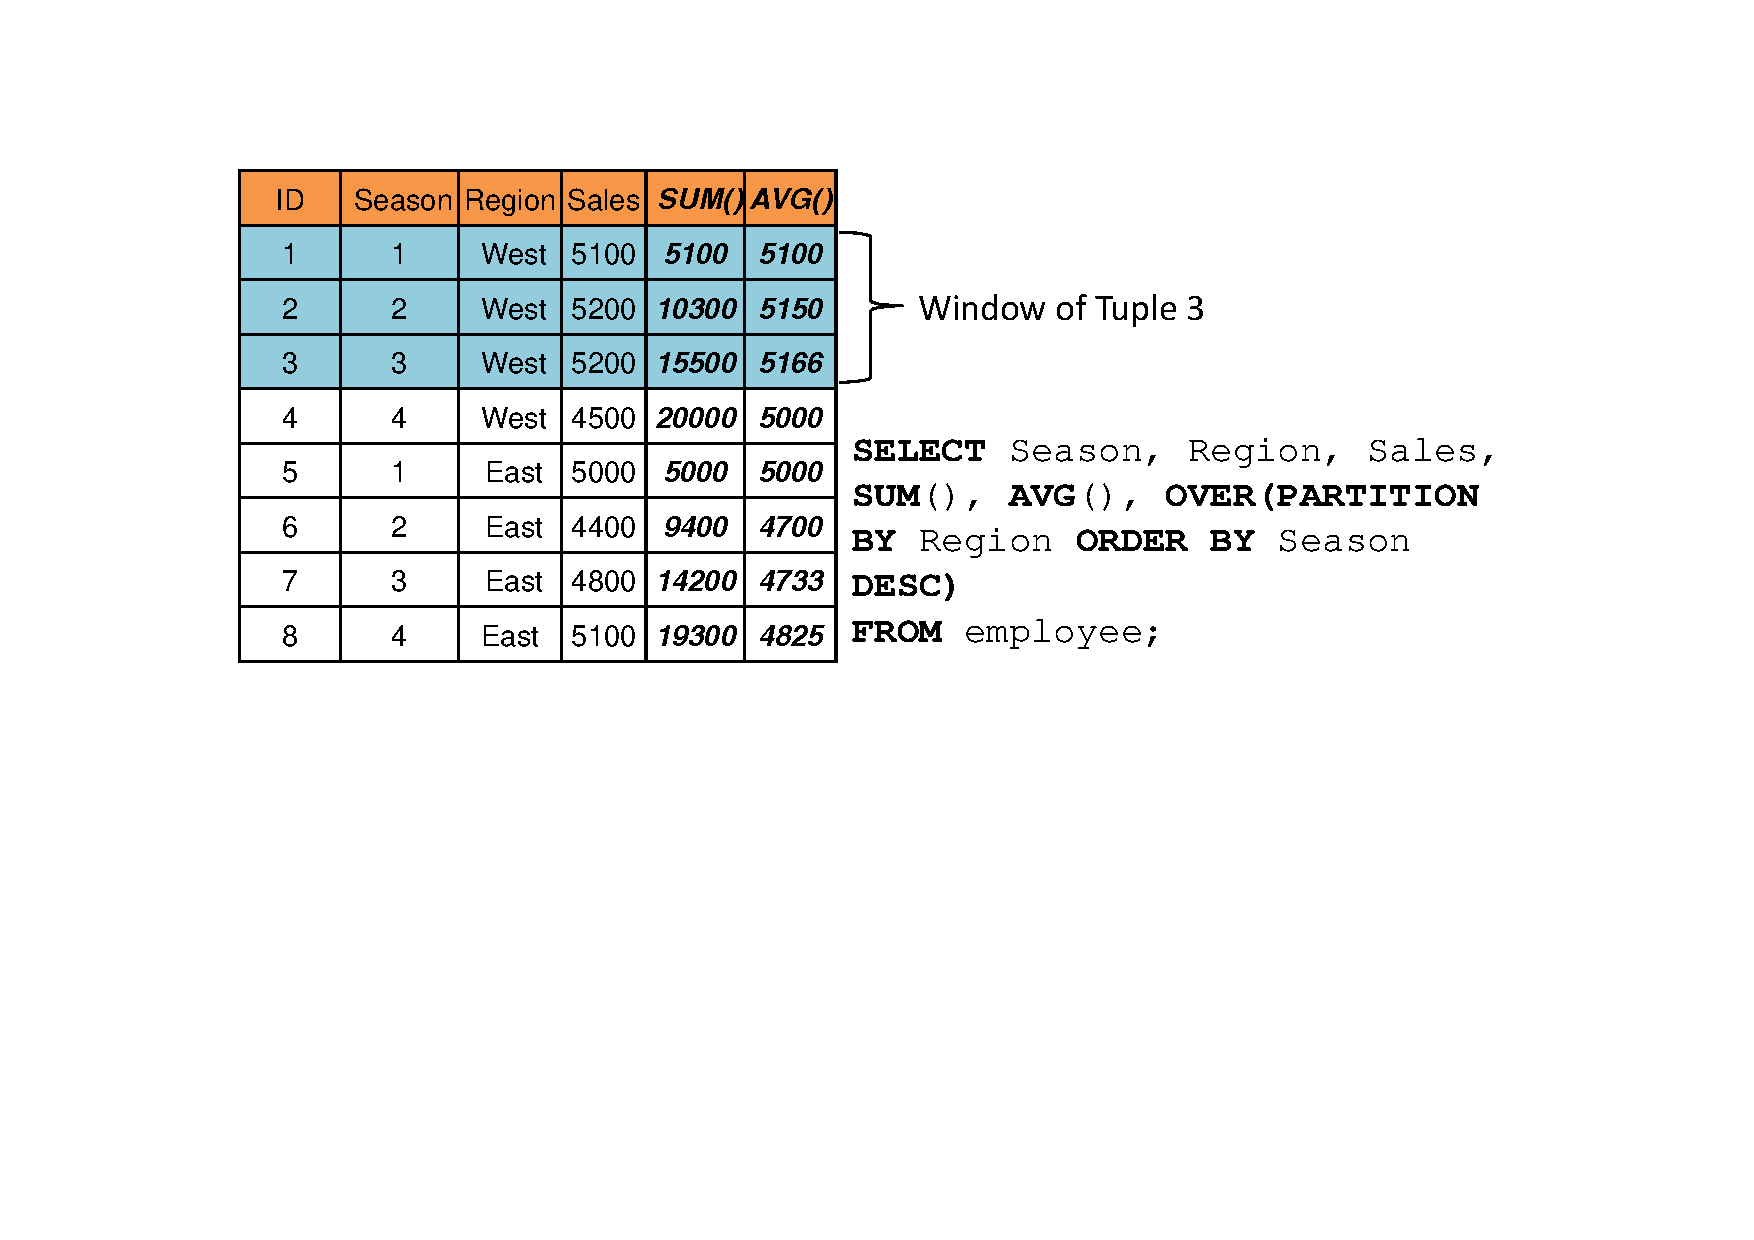
\includegraphics[width=0.8\linewidth]{window_example.pdf}
\caption{A SQL window function computing running sum and average of
sales. The window of tuple 3 is highlighted.} 
\label{fig:window}
\end{figure}

As shown in the figure, the sales report contains six columns: ``ID'',
``Season'', ``Region'' and ``Sales'' are the \emph{facts}, ``$\mathtt{sum()}$'' and ``$\mathtt{avg()}$''
are the \emph{analytics} representing the running sum and average. A window function
is represented by the $\mathtt{over}$ keyword. In this context, the window of a tuple $o_i$
contains another tuple $o_j$ if $o_i$ and $o_j$ are in the same ``region'' and the``season'' of $o_j$ is
prior to the season of $o_i$. The window of tuple-$3$ is highlighted.
Apart from this example, there are also many other 
usages of the window functions in the relational context~\cite{cao2012optimization}. 
Being aware of the success of the window functions, 
SQL~11~\cite{zemke2012s} standard incorporates ``$\mathtt{LEAD}$'' and ``$\mathtt{LAG}$'' 
keywords to offer fine-grained specifications on a tuple's window.

Despite the usefulness, there are few works reporting
the usage of window functions in data domains such as graphs, sequence data and trajectories.
This may be due to the
requirement of \emph{sorting} in the window functions. For example,
in Figure~\ref{fig:window},
objects need to be sorted according to ``Season'', and then the window of
each object is implicitly formed based on the sorted order. However, 
in domains like graphs and time series data, sorting may be ambiguous and even undefined.

To broaden the usages of the window functions in other data domains, we propose the \emph{neighborhood
analytics} in a more general sense. Given a set of objects 
(such as tuples in relational tables, vertexes in graphs, moving objects in trajectories),
the neighborhood analytics is a composite function
$(\mathcal{F} \circ \mathcal{N})$ applied on every object. Here, $\mathcal{N}$
is the \emph{neighborhood function}, which contains the related objects (i.e., vicinity) of an object;
$\mathcal{F}$ is the \emph{analytic function}, which could be aggregation, ranking,
pattern matching, etc.
Apparently, the SQL window function is a special case of the
neighborhood analytics. For example, the window function in Figure~\ref{fig:window} 
can be represented as $\mathcal{N}(o_i)=\{o_j | o_i.season > o_j.season \wedge o_i.region = o_j.region\}$
and $\mathcal{F} = \mathtt{avg}$.
By relaxing the sorting constraint, neighborhood analytics gains an enriched 
semantic and can be applied on many other data domains.

%Since the \emph{sorting} requirement is relaxed, our neighborhood analytics is able to
%enrich the semantic of relational window notations 
%and can be applied on many other domains.